\section{Results}

\begin{figure*}[!t]
  \centering
  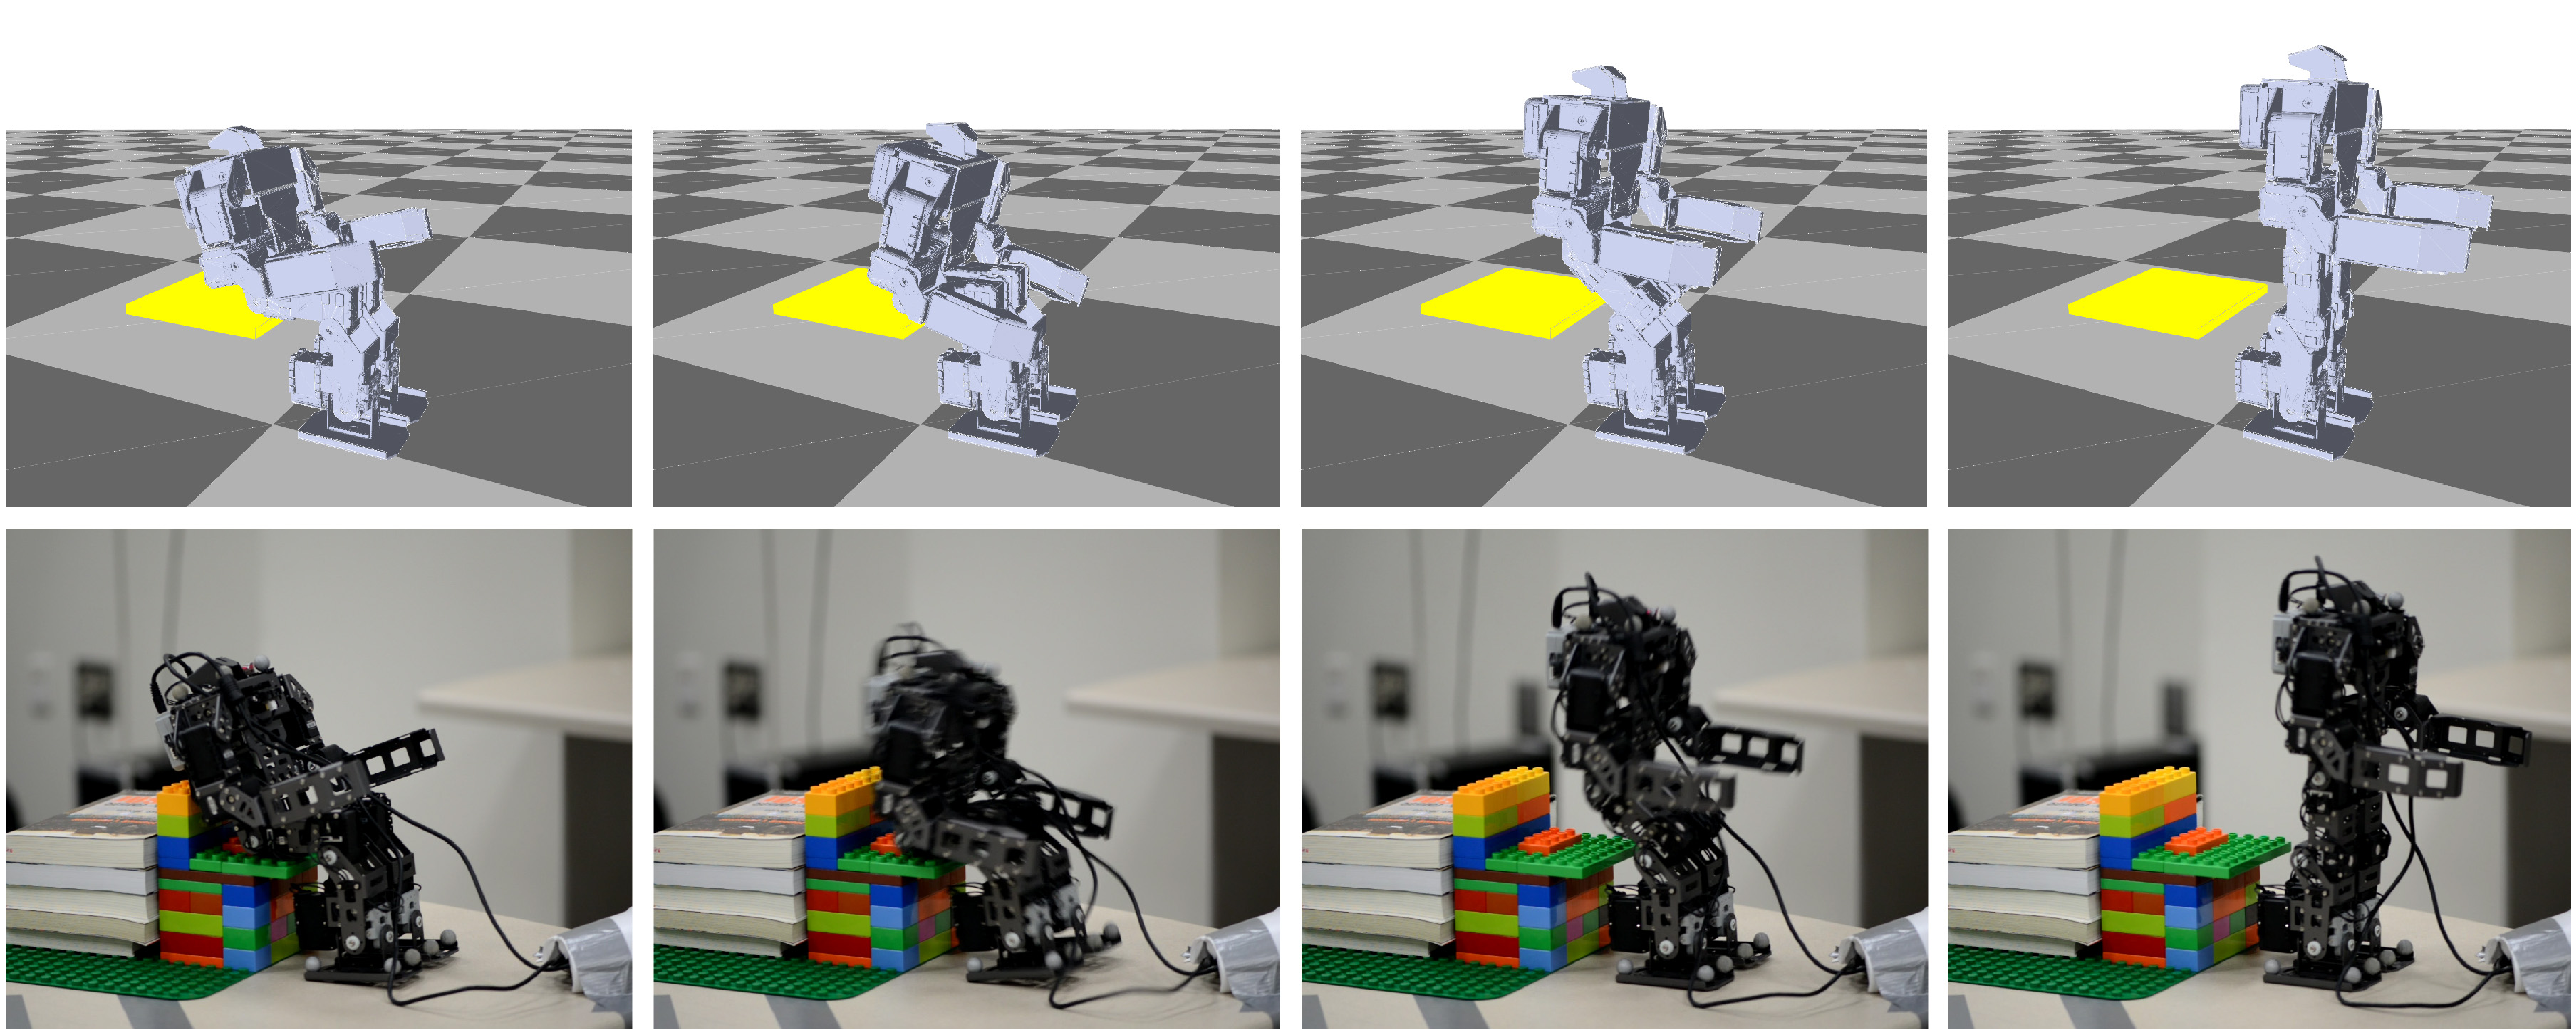
\includegraphics[width=\textwidth]{figures/sit2Stand}
  \caption{The results of the sit-to-stand task in the simulation and on the real robot.}
  \label{fig:sit2Stand}
\end{figure*}

In this section we present the results of our system. We use four locomotion tasks to evaluate our system: The robot rises from a leaning, sitting or kneeling position and flipping to a handstand pose. Please watch the accompanying video for the robot performance in the simulation and in the real world.

\subsection{Experiment Setup}

We use BIOLOID GP as our robot platform. BIOLOID GP is a humanoid robot that consists of 18 degrees of freedom that are powered by Dynamixel AX-12/AX-18 servos. The communication between the PC and the robot is through a serial port. To control the robot, a master program on the PC writes the desired pose $\bar{\mathbf{q}}$ to the serial port that is connected to the robot. A slave program that runs on the robot's onboard microprocessor listens to this port and sends the desired joint angle to each actuator. At the same time, the robot performance data $\tilde{\mathbf{x}}$ is measured and sent back to the computer. We use onboard rotary encoders to measure joint angles and a VICON motion capture system to measure the global position and orientation of the robot's torso. The average latency of the whole control loop on our robot is 16ms. It is measured by a timer in our program between the time when the master program starts sending the actuator commands to the robot and when it finishes reading the sensor measurements from the robot.

\subsection{Implementation Details}

Our system is implemented in C++ and runs on a laptop with a 2.6GHz quad-core CPU and 16GB of memory. We use DART to simulate the physics of the robot and its surrounding environments. In our work, we initialize the simulation parameters as follows. We set the physical properties of each body segment, including the mass, the moment of inertia and the COM according to the CAD files. We set the actuator gains based on the measurement from experiments (Section \ref{sec:motorDynamics}). We leave all other parameters as default values in DART. Although these parameters are not accurate, they serve as a good initial guess. We use 1ms as the time step in physical simulation. We recompute the control signal every 16 time steps in the simulation to mimic the actual control latency on the robot.

We find that all four tasks can be achieved with symmetric lower body motions. This observation enables us to reduce the dimensionality of the control space. In controller optimization, we halve the size of the optimization problem by exploiting this symmetry of the motion. We constrain that the joint motions on the left bodies mirror those on the right bodies. In addition, we also constrain our optimization to the lower body motions.

During simulation calibration, we search for the simulation parameters within a bounded range centered at their initial settings. Although there are dozens of simulation parameters that can be calibrated at this stage, we choose to focus on the COM of each body segment and the actuator gains since they are the most relevant parameters to the success of our locomotion tasks. In all the experiments, we choose the weights $\mathbf{W}$ in the objective function (eq. (\ref{eqn:calibrationObj})) such that $E_{cali}$ measures the difference of the global orientations of the root body between in the simulation and in the real world. For each simulation calibration, we collect three episodes of robot data by running the same controller three times to average out the noise and initial condition perturbations. Each episode is approximately two seconds.

The parameter settings of CMA for both controller optimization and simulation calibration are the same. We use 32 CMA samples per iteration and at most 50 iterations. We distribute the computation across all four cores of the CPU. It takes less than 15 minutes to find an optimal solution in controller optimization or simulation calibration.

\begin{figure}[!t]
  \centering
  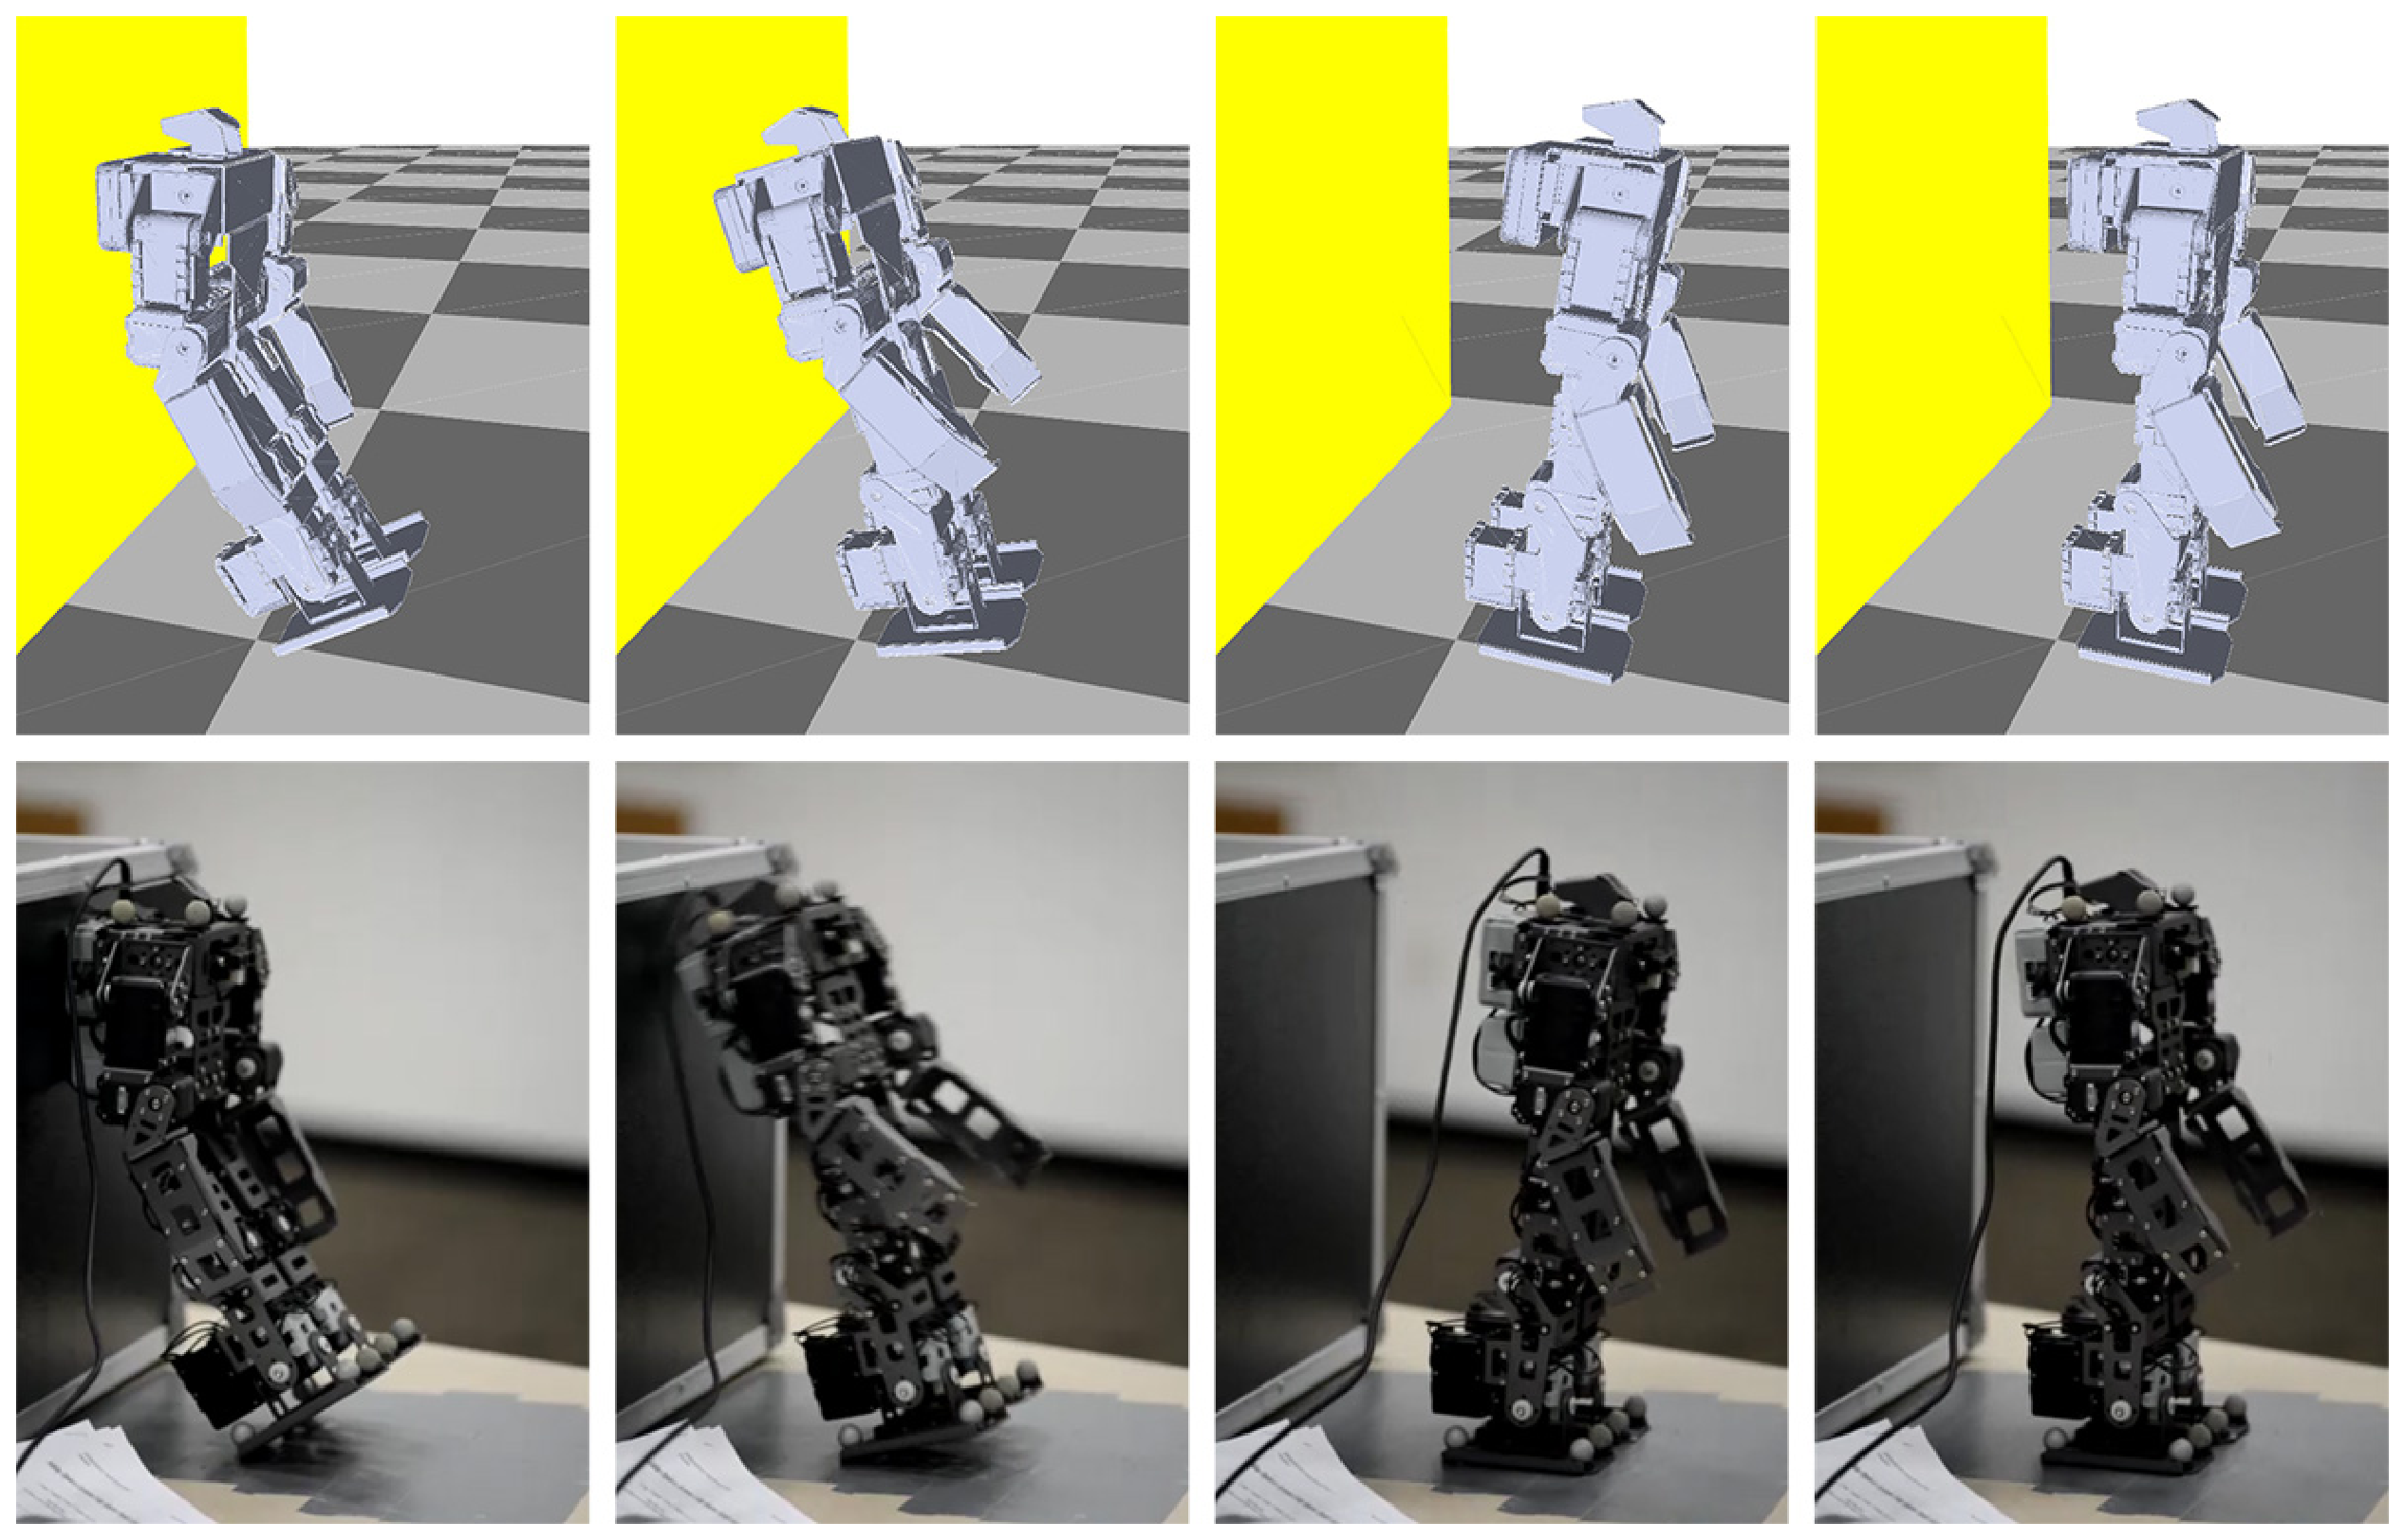
\includegraphics[width=0.5\textwidth]{figures/lean2Stand}
  \caption{The results of the lean-to-stand task in the simulation and on the real robot.}
  \label{fig:lean2Stand}
\end{figure}

\subsection{Rising from a Sitting Position}

The first task that we have tested is to rise from a sitting pose to a standing pose (Figure \ref{fig:sit2Stand}). The initial and the final poses $q_0$ and $q_T$ are shown in the leftmost and rightmost images in Figure \ref{fig:sit2Stand}. The controller optimization needs to search for an additional inbetween keyframe $q_1$, as well as the two time intervals $t_1$ and $t_2$ between these three keyframes. 

We intentionally choose the initial pose that the legs of the robot extend forward and the projection of the robot's COM in the vertical direction falls far behind the contact points of the feet. If the robot simply extends the hips and the knees to stand up, it will fall backwards. Despite this challenging setup, our system successfully finds a controller that enables the robot to stand up in the simulation. Figure \ref{fig:sit2Stand} shows that the robot first builds up a forward momentum by quickly leaning its upper body to the front. It then starts to extend the hips and the knees at the moment when the COM is approaching the boundary of the support polygon spanned by the feet. This effective standing-up strategy is found automatically by the controller optimization subsystem.

When applying this controller to the real robot, we are surprised to find that it works directly, without the need of simulation calibration. The robot stands up from a chair in the same way as its simulated counterpart does in the virtual world. This shows that the Reality Gap is not always a problem. In some tasks, the stability region of a controller is so large that it can make the discrepancy between the virtual and the real world less critical.

\subsection{Rising from a Leaning Position}

In this task, the robot needs to rise from leaning on the wall to a standing position (Figure \ref{fig:lean2Stand}). In the initial configuration, the hip joints are bent and they are straightened out in the final configuration while all other joints do not move. The initial and the final poses are the only two keyframes for this task.

\begin{figure}[!b]
  \centering
  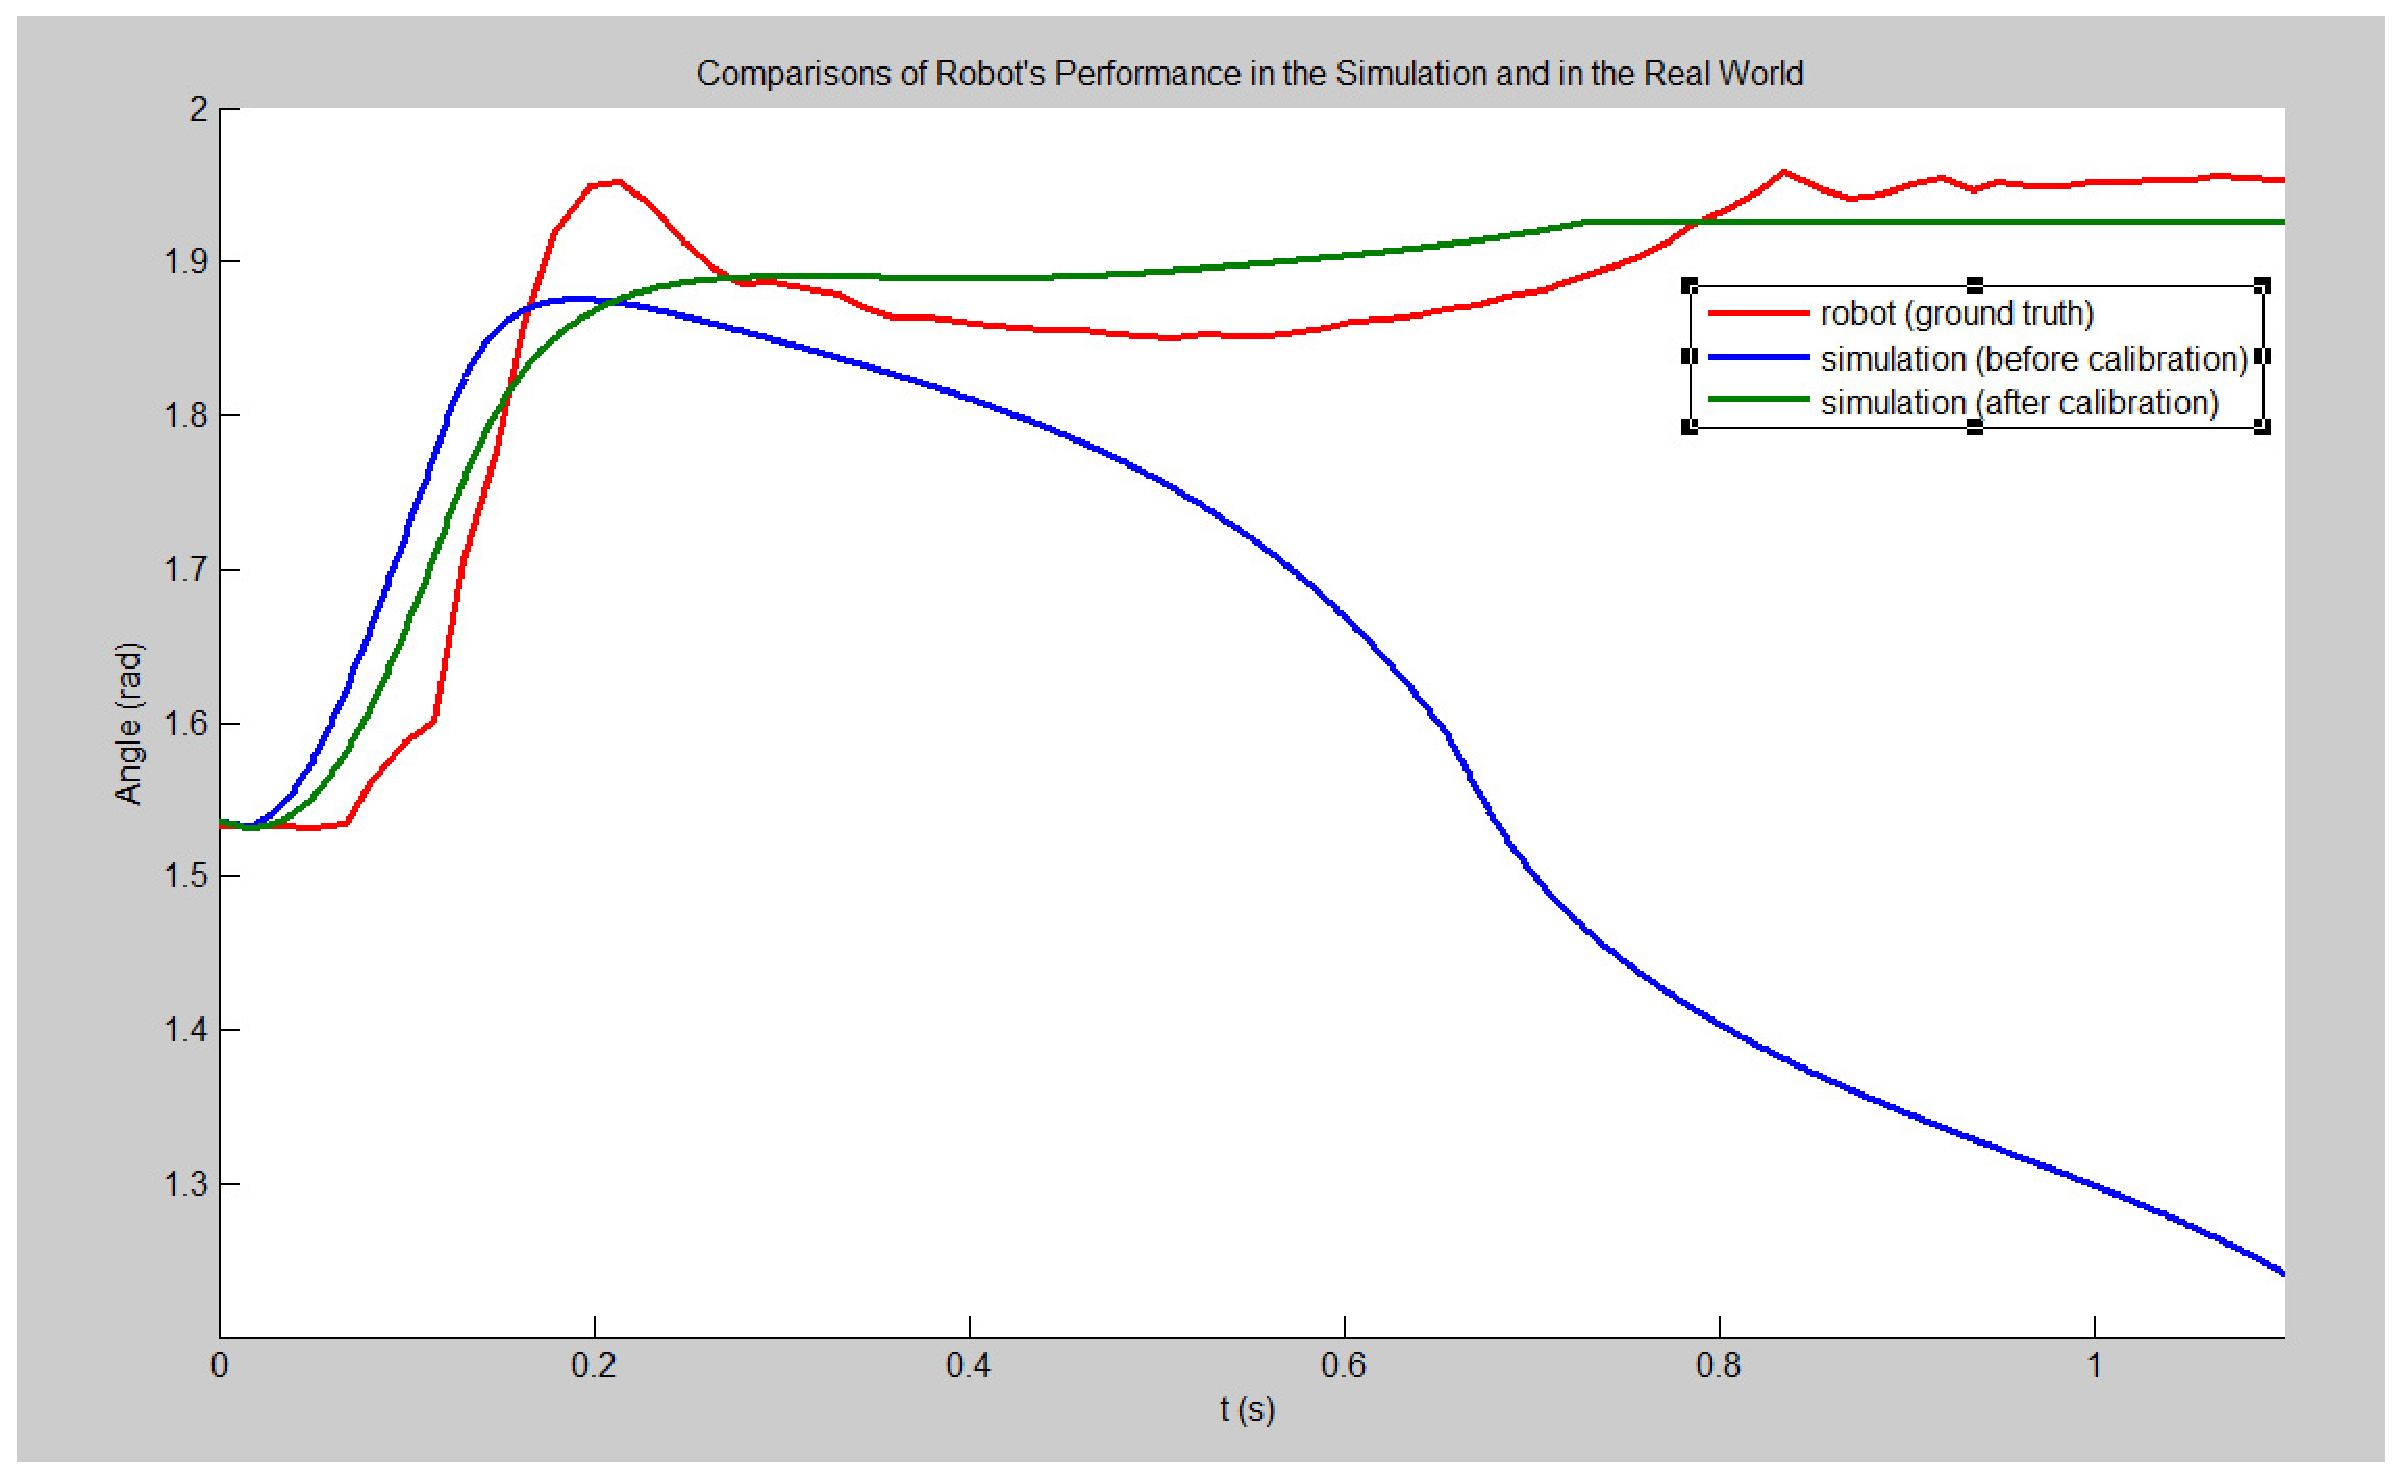
\includegraphics[width=0.4\textwidth]{figures/simRobotCompare}
  \caption{Comparisons of the robot's global orientation over time in the simulation (before/after calibration) and in the real environment.}
  \label{fig:simRobotCompare}
\end{figure}


The goal of controller optimization is to find an appropriate time interval $T$ between these two keyframes. If the time interval is too long, the robot moves slowly, and cannot accumulate enough momentum to rise. If this time interval is too short, the robot move abruptly, which will cause the upper body to bounce off the wall too quickly and fall forward. Without simulation calibration, the controller optimization cannot find a working controller for this task. The robot cannot rise when $T\leq 0.10s$ and overshoots when $T > 0.10s$. Nevertheless, we apply the controller with the highest fitness value $T=0.11s$ on the robot. In contrast to the simulation result, in which the simulated robot rises too quickly and falls forward, the robot in the real world actually cannot rise. Figure \ref{fig:simRobotCompare} compares the trajectories of the robot's global orientation in the simulation (blue curve) and in the real world (red curve). After one iteration of simulation calibration, the discrepancy is greatly reduced (Figure \ref{fig:simRobotCompare} green curve). We optimize the controller again in this calibrated simulator. This time, the optimal controller works both in the simulated and in the real world.

\begin{figure}[!b]
  \centering
  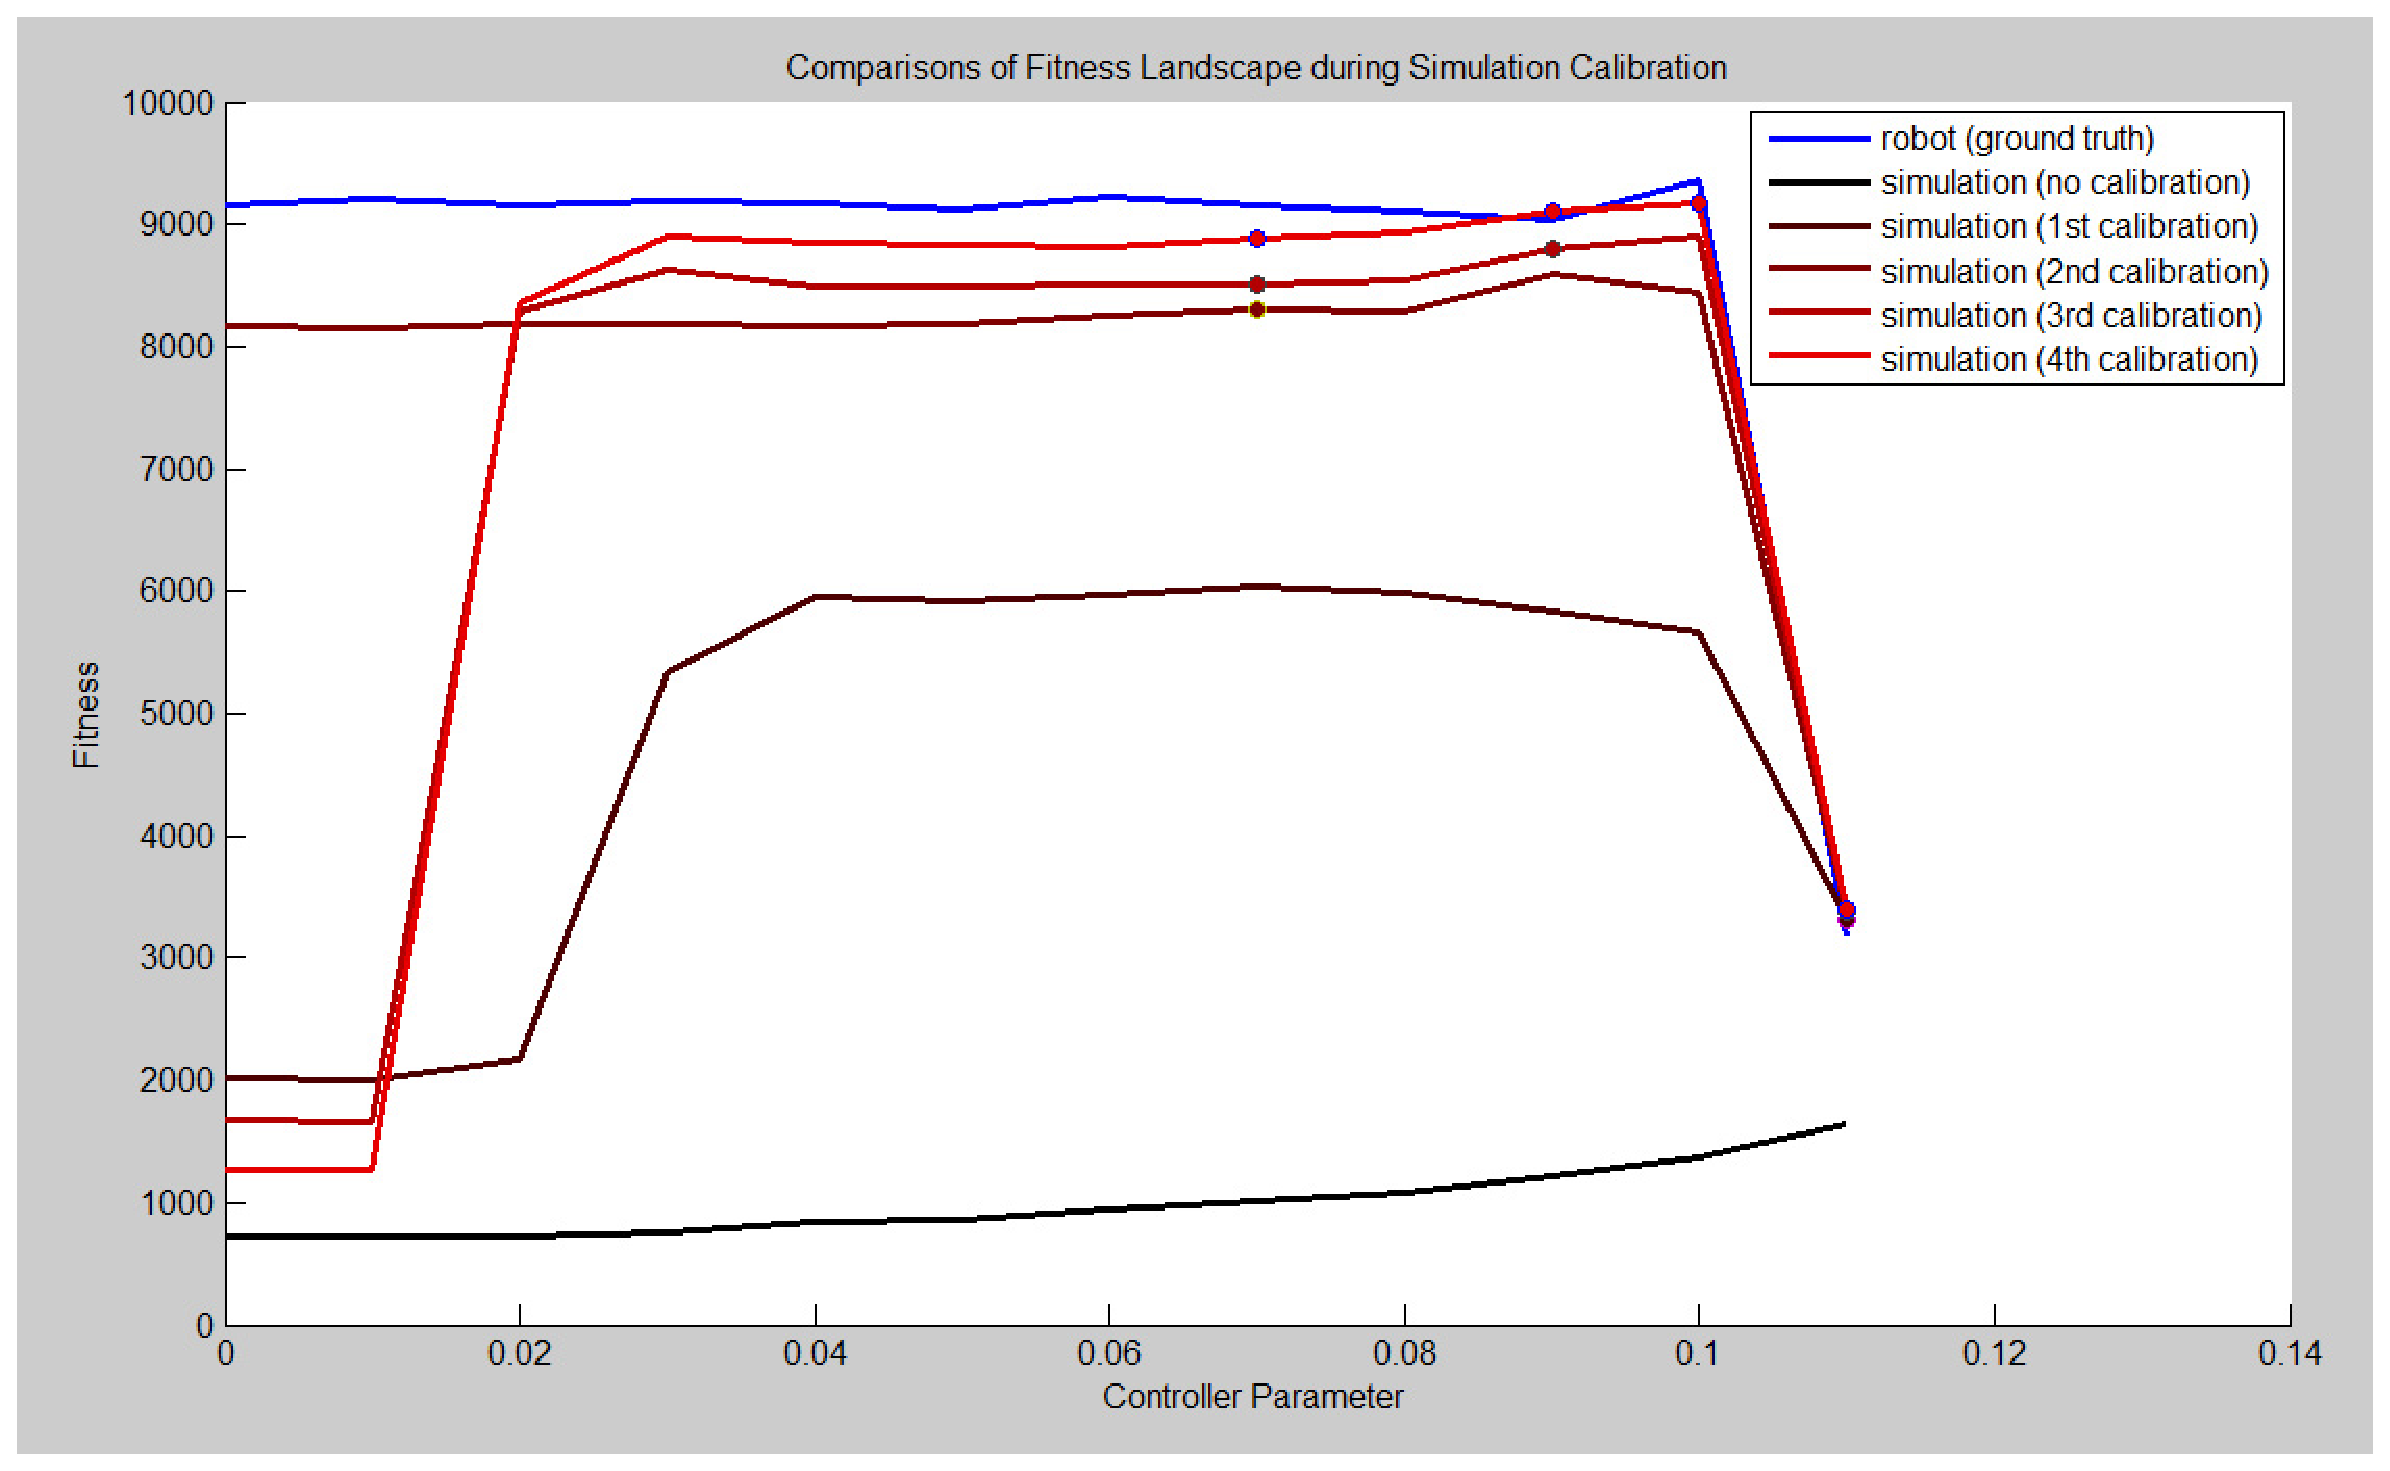
\includegraphics[width=0.4\textwidth]{figures/fitnessLandscape}
  \caption{Comparisons of the fitness landscape as more iterations of simulation calibration are performed.}
  \label{fig:fitnessLandscape}
\end{figure}

\begin{figure*}[!t]
  \centering
  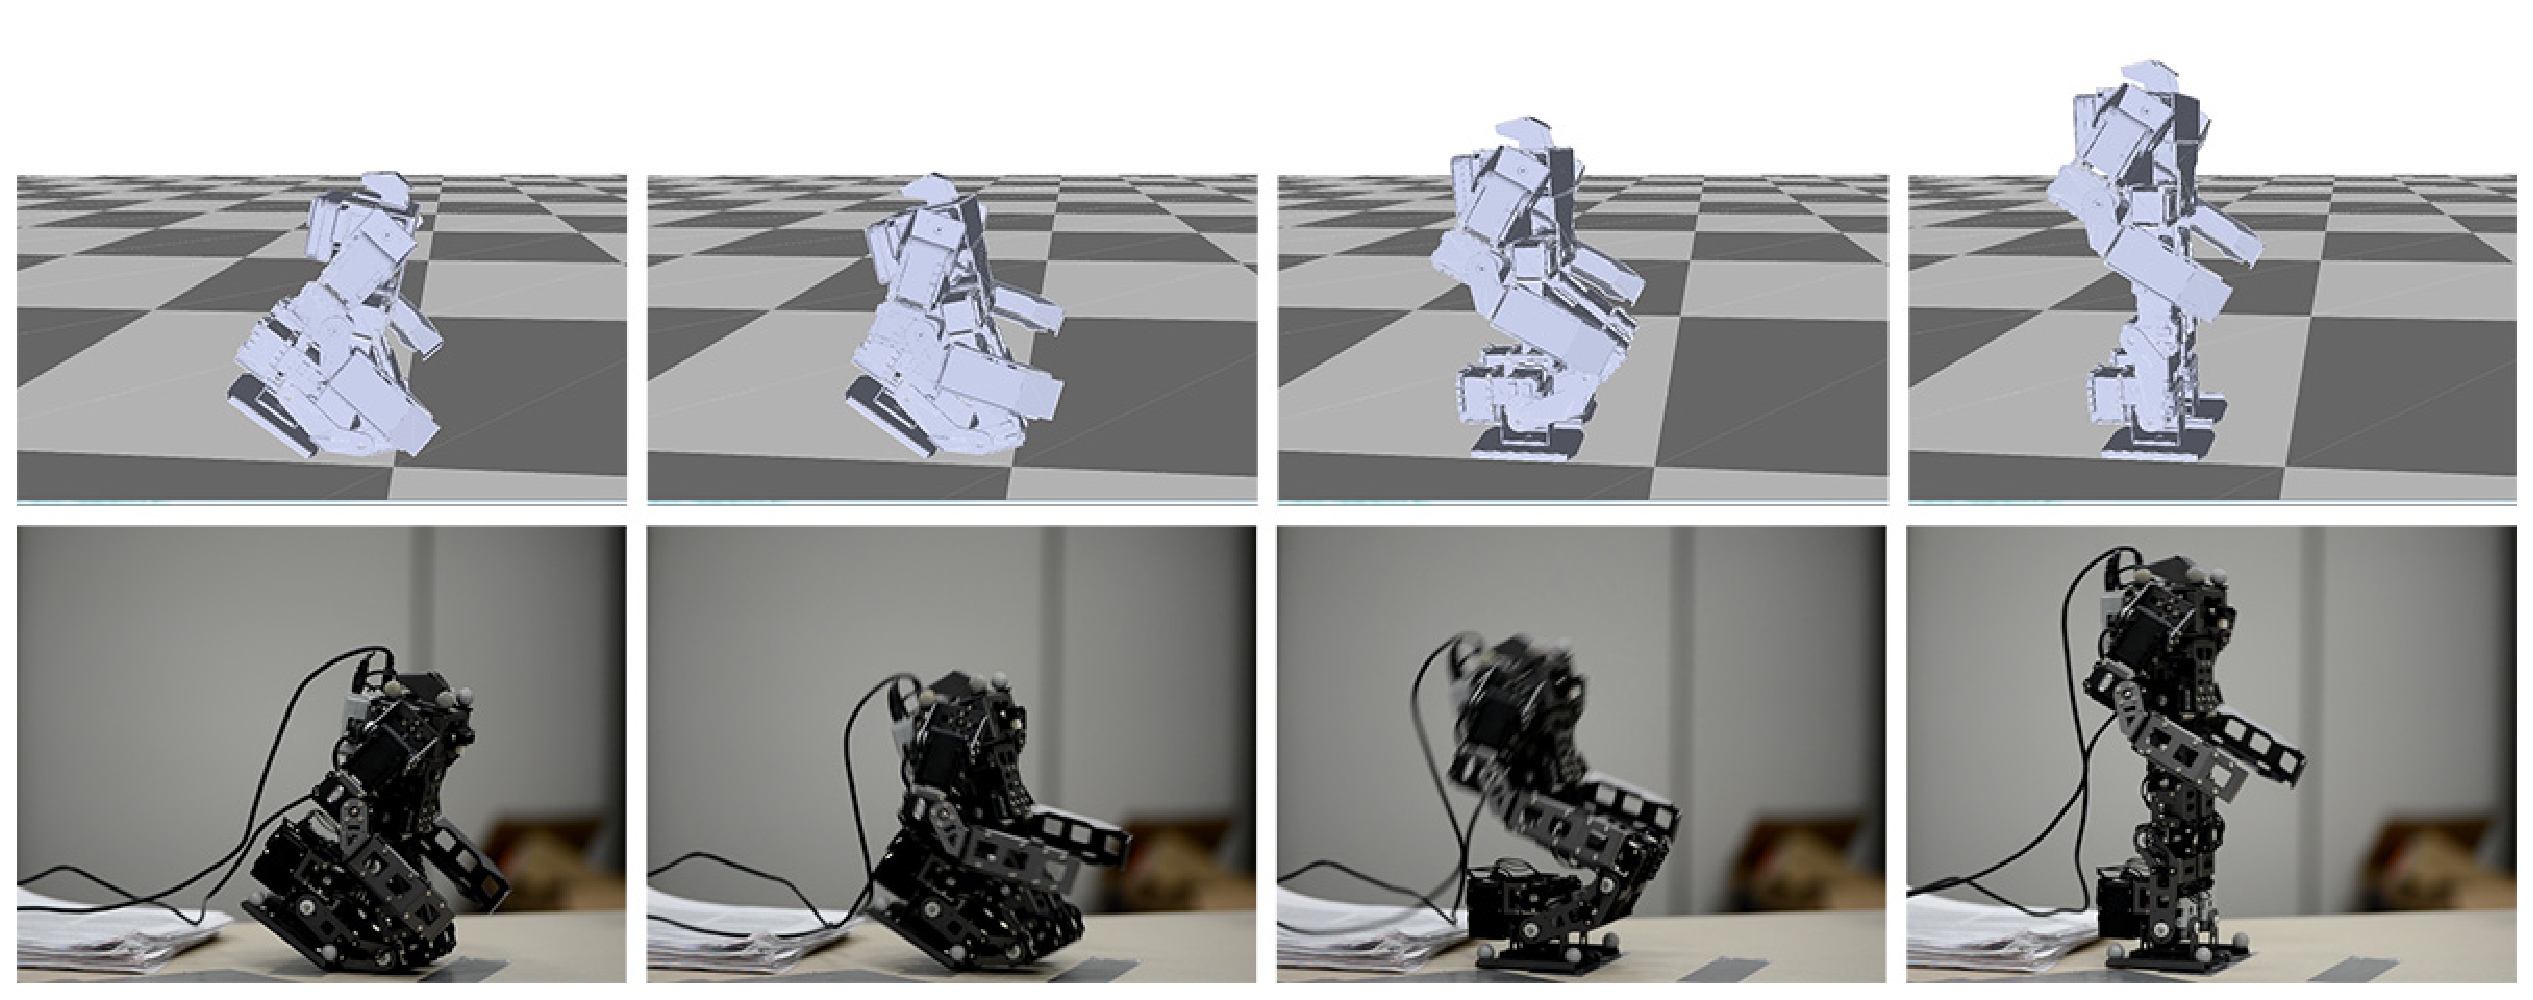
\includegraphics[width=\textwidth]{figures/kneel2Stand}
  \caption{The results of the kneel-to-stand task in the simulation and on the real robot.}
  \label{fig:kneel2Stand}
\end{figure*}

We successfully cross the Reality Gap with one iteration of simulation calibration, which uses only three episodes of robot experiments and totally 6 seconds of robot data. To better understand how the Reality Gap is gradually narrowed by simulation calibration over multiple iterations, we perform an additional evaluation. Figure \ref{fig:fitnessLandscape} shows how the fitness landscape in the simulation changes with different number of iterations of simulation calibration. The blue curve is the ground truth. It is evaluated on the real robot by varying the control parameter $T$ in the range of $[0, 0.11]$. The fitness value is calculated according to eq. (\ref{eqn:controllerObj}). The fitness landscape stays at a high value when $T\in[0, 0.1]$, which means that the real robot can successfully rise if the controller uses less than 0.1s to change the pose from the initial to the final configuration. In contrast, without simulation calibration, the fitness landscape (lowest black curve) stays at a low value for the entire control space. In other words, no controller exists that can make the robot stand up in the simulation. The gap between the blue and the black curves is analogue to the Reality Gap. One iteration of simulation calibration brings the fitness landscape in the simulation towards the ground truth. As more iterations are performed, the fitness landscape in the simulation (brown and red curves) gradually approaches the ground truth, and the Reality Gap is narrowed in this process. Note that a large discrepancy still exists in the region of the parameter space where $T<0.02s$. This is probably caused by two reasons. First, in the region of $T<0.02s$, the torque output of the servo is at its limit but the torque limit is not considered in simulation calibration. Second, the controllers and the data (the red circles in Figure \ref{fig:fitnessLandscape}) that we use in simulation calibration concentrate on the right half of the parameter space, which makes it difficult to generalize to a region where the data is scarce ($T<0.02$). However, this is beneficial in our applications because the computational resource is focused at the important regions near the successful controllers. This explains why our system can find a successful controller in the real word with minimal robot experiments.

\subsection{Rising from a Kneeling Position}

Figure \ref{fig:kneel2Stand} shows that the robot stands up from a kneeling pose. Between the user-specified initial and final poses, the controller consists of two additional keyframes. The optimization needs to search for these keyframes and the time intervals between adjacent keyframes. The controller optimized in the simulation demonstrates an agile getting-up motion: The robot first leans its upper-body backwards. As its COM is moving to the back, it quickly bends the hip, flexes its ankles and stands up. This entire motion resembles one of the most agile ways that we human get up from a kneeling position when we do not use our hands for additional support. Although this controller works perfectly in the simulation, the robot falls backward in the real world. After simulation calibration, the performance of the simulated robot comes closer to the real world scenario. Using the calibrated simulator, we optimize a new controller, with which the robot can successfully stand up from the kneeling position in the real world (Figure \ref{fig:kneel2Stand}).

\begin{figure*}[!t]
  \centering
  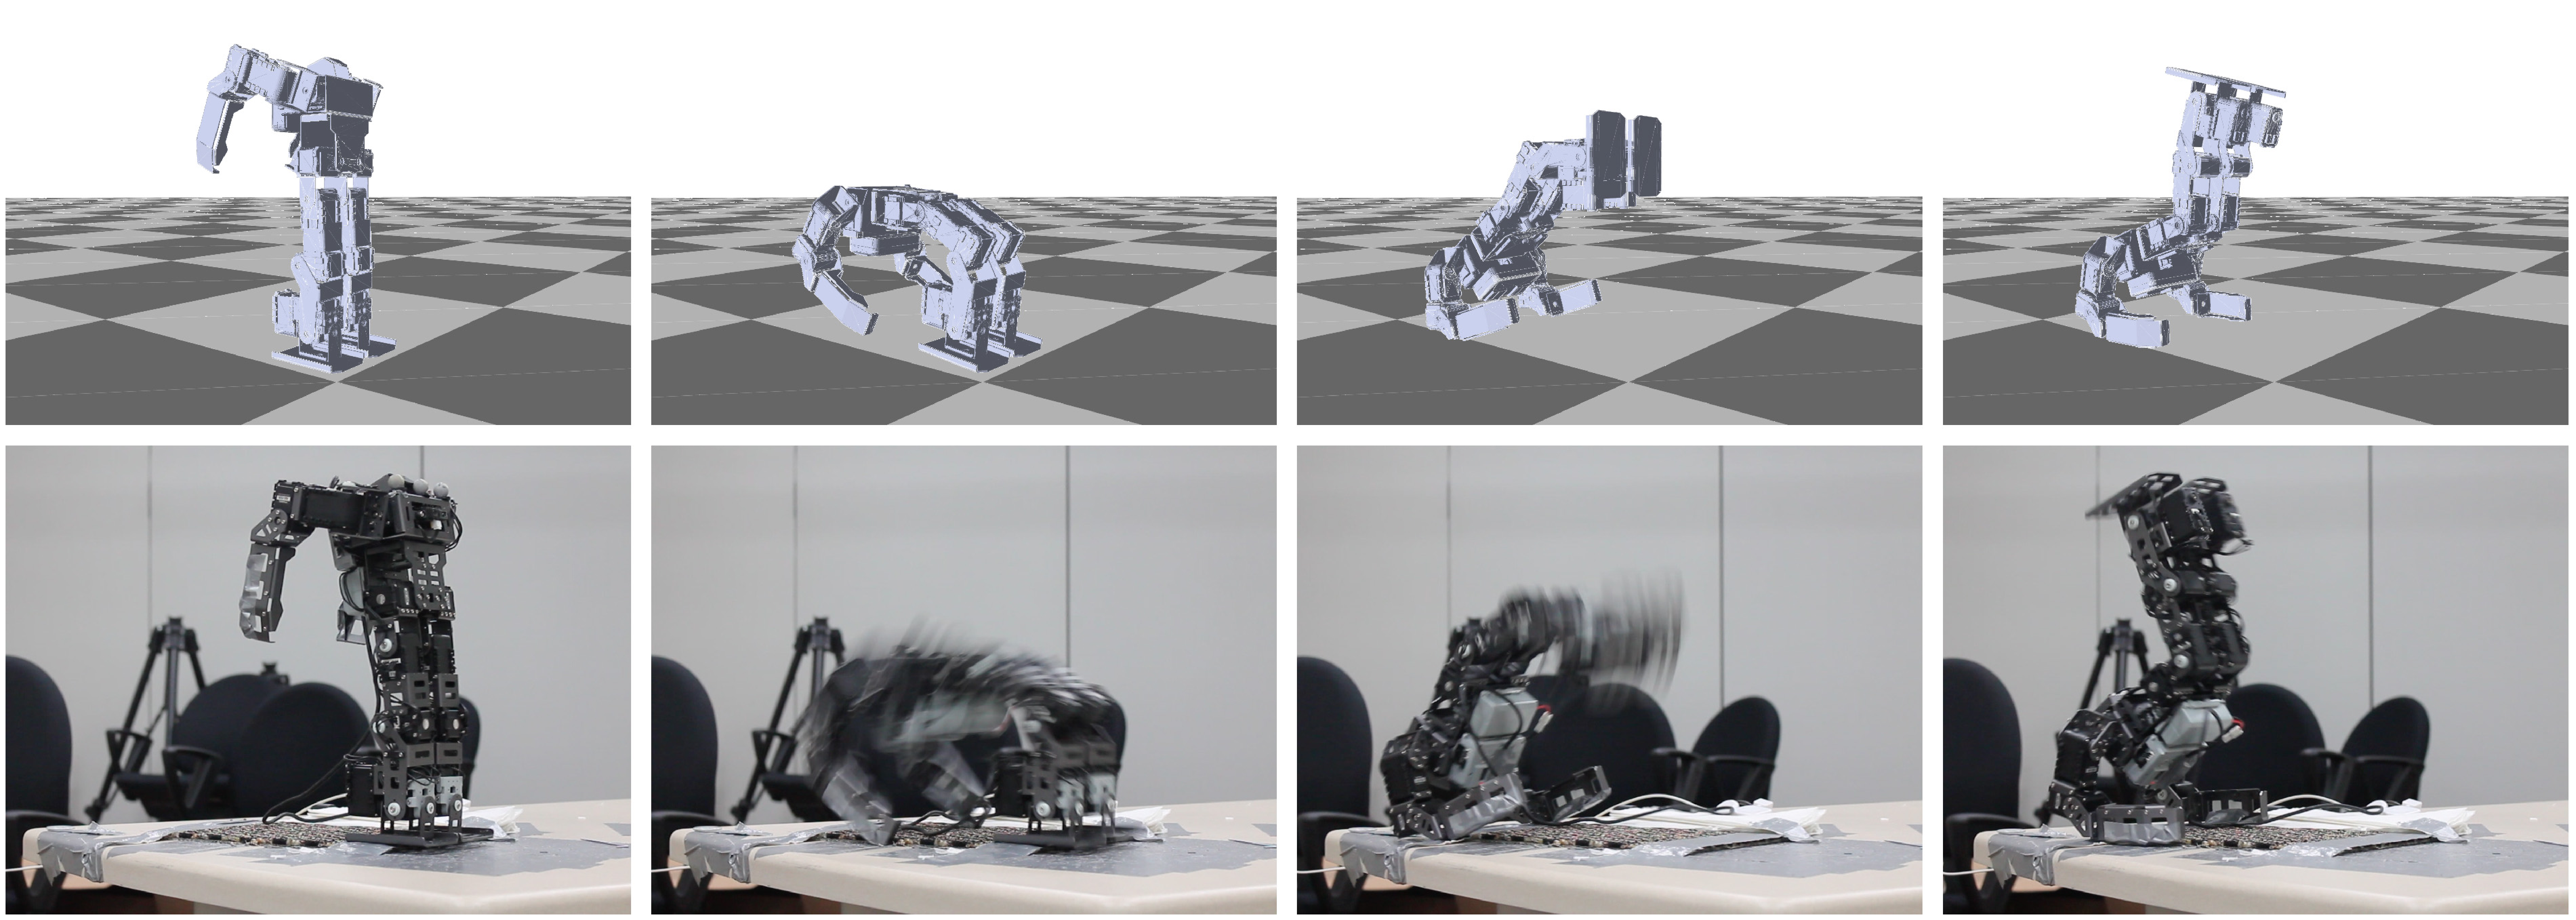
\includegraphics[width=\textwidth]{figures/stand2Hand}
  \caption{The results of the stand-to-handstand task in the simulation and on the real robot.}
  \label{fig:stand2Hand}
\end{figure*}


\subsection{Flipping to a Handstand Position}
We test our system with a more challenging task: flipping to a handstand position from a standing pose, which is often seen in gymnastics. The initial and final poses are shown in Figure~\ref{fig:stand2Hand}. The controller optimization needs to search for an additional keyframe between them. Without simulation calibration, controller optimization cannot find a controller to fulfil this task in the simulation. Nevertheless, we apply the controller with the highest fitness value to the robot to collect data for simulation calibration. After two iterations of simulation calibration and controller optimization, our system finds a successful controller that works both in the simulation and in the real world: The robot arches back rapidly and lifts its feet after the arms touch the ground. Both the speed and the curvature of the arching motion is crucial for the final balance. Although only a narrow range of such speed and curvature can lead to a balanced handstand, our system is able to automatically find a successful controller for this challenging task.

